% -*- program: xelatex -*-

\documentclass[12pt, t]{beamer}
%%% ------------------------------------------------------------------------
% packages
\usepackage{tikz}
\usetikzlibrary{shapes.geometric, arrows, positioning, shapes, backgrounds}
\usepackage{graphicx}
\usepackage{lmodern}
\usepackage{adjustbox}
% conditional (for figures)
\usepackage{etoolbox}
% \usepackage{listings}
\usepackage{minted}

\usepackage{fontspec}
\usepackage{fontawesome}

\usepackage{subcaption} % side-by-side figures
\usepackage{hyperref}



%%% ------------------------------------------------------------------------
% Theming (dark or white)
\usetheme{default}
\useoutertheme[subsection=false]{miniframes}

% move navigation to footer
\setbeamertemplate{headline}{}
\makeatletter
\setbeamertemplate{footline}
  {%
  \begin{beamercolorbox}{section in head/foot}
    \vskip2pt\insertnavigation{\paperwidth}\vskip5pt
  \end{beamercolorbox}%
  }
\makeatother


% no navigation bar
\beamertemplatenavigationsymbolsempty

% switch between white and black
\newtoggle{dark}
\toggletrue{dark}
% \togglefalse{dark}

\iftoggle{dark}{%
    % some colors
    \definecolor{foreground}{RGB}{255,255,255}
    \definecolor{background}{RGB}{24,24,24}
    \definecolor{title}{RGB}{127,185,220}
    \definecolor{gray}{RGB}{116,116,116}
    \definecolor{hilight}{RGB}{250, 108, 0}
    \setbeamercolor{section in head/foot}{fg = title}
    % set colors for titles, etc.
    \setbeamercolor{titlelike}{fg=title}
    \setbeamercolor{subtitle}{fg=title}
    \setbeamercolor{institute}{fg=gray}
    \setbeamercolor{normal text}{fg=foreground,bg=background}
    % % set colors for itemize
    \setbeamercolor{item}{fg=title} % color of bullets
    \setbeamercolor{subitem}{fg=gray}
    \setbeamercolor{itemize/enumerate subbody}{fg=gray}
}{
    % some colors
    \definecolor{foreground}{RGB}{0, 0, 0}
    \definecolor{background}{RGB}{255,255,255}
    \definecolor{title}{RGB}{107,174,214}
    \definecolor{gray}{RGB}{116,116,116}
    \definecolor{hilight}{RGB}{228, 97, 0}
    \setbeamercolor{section in head/foot}{fg = title}
    % set colors
    \setbeamercolor{titlelike}{fg=title}
    \setbeamercolor{subtitle}{fg=title}
    \setbeamercolor{institute}{fg=gray}
    \setbeamercolor{normal text}{fg=foreground,bg=background}
    % set colors for itemize
    \setbeamercolor{item}{fg=foreground} % color of bullets
    \setbeamercolor{subitem}{fg=gray}
    \setbeamercolor{itemize/enumerate subbody}{fg=gray}
}


%%% -----------------------------------------------------------------------


%%% ------------------------------------------------------------------------
% Meta
\title{Web Scraping with R}   
\author{Eduard Szöcs} 
\institute{Institute for Environmental Sciences, University of Koblenz-Landau} 
\date{Landau, 25.02.2016}



%%% ------------------------------------------------------------------------
% Title page
\begin{document}

\begin{frame}
\titlepage
\end{frame}


%%% ------------------------------------------------------------------------
% Intro
\section{About me} 
\subsection{}
\begin{frame}
\frametitle{About me}
\begin{itemize}
\item Phd-Student @Uni Koblenz-Landau
	\begin{itemize}
	\item Environmental monitoring data
	\end{itemize}
\item Freelance R Consultant
	\begin{itemize}
		\item R Courses
		\item Data sourcing, cleaning \& analysis
	\end{itemize}
\end{itemize}
\pause
\vspace{2em}
R packages:
\begin{description}
	\item[\href{https://github.com/ropensci/taxize}{taxize}]{Taxonomic Information from Around the Web}
	\item[\href{https://github.com/ropensci/webchem}{webchem}]{Chemical Information from the Web}
\end{description}
\begin{centering}
\colorbox{white}{
\includegraphics[width =.3\textwidth]{fig/ropensci.png}}
\end{centering}
\end{frame}


\section{Tools}
\subsection{}
\begin{frame}
\frametitle{I - Packages (selected)}
\begin{description}
\item[\textcolor{hilight}{xml2}]{Parsing XML \& HTML}	
\item[\textcolor{hilight}{rvest}]{parse common html structures (e.g. tables)}
\item[\textcolor{hilight}{xmlview}]{View pretty HTML/XML, explore XPaths}
\item[httr*]{Working with APIs / http protocol}
\item[jsonlite*]{Parse JSON}
\end{description}
\pause

\includegraphics[width=.3\textwidth]{fig/adcr-cover-wiley4.jpg} \\
\tiny
* I won't cover APIs here.
\end{frame}


\section{structured webpages}
\subsection{}
\begin{frame}[fragile]
\frametitle{II - Scraping structured web-pages}
What is structured?
\begin{minted}[fontsize=\tiny]{html}
<table class="wikitable">
  <tbody>
    <tr>
      <th>First name</th>
      <th>Last name</th>
      <th>Age</th>
    </tr>
    <tr>
      <td>Tinu</td>
      <td>Elejogun</td>
      <td>14</td>
    </tr>
    <tr>
      <td>Blaszczyk</td>
      <td>Kostrzewski</td>
      <td>25</td>
    </tr>
    [...]
  </tbody>
</table>
\end{minted}
2D representation of data -> data.frame
\end{frame}


\begin{frame}
\frametitle{II - Demo}
Extract election results from wikipedia \\
\tiny
\url{https://de.wikipedia.org/wiki/Landtagswahlen_in_Rheinland-Pfalz}

\vspace{1em}
\begin{adjustbox}{max totalsize={.9\textwidth}{.7\textheight},center}
\begin{tikzpicture}[node distance = 1cm, auto]
\tikzstyle{block} = [rectangle, draw, fill=title, text = black,
    text width=8em, text centered, rounded corners, minimum height=4em]
\tikzstyle{line} = [draw, thick, -latex']
    % Place nodes
    \node [block] (source) {Look at the source};
    \node [block, right=of source] (download) {download \\ xml2::read\_html()};
    \node [block, right=of download] (parse) {parse \\ rvest::html\_table()};
    \node [block, right=of parse] (clean) {clean / use};

%paths
    \path [line] (source) -- (download);
    \path [line] (download) -- (parse);
    \path [line] (parse) -- (clean);

\end{tikzpicture}
\end{adjustbox}
\vspace{2em}

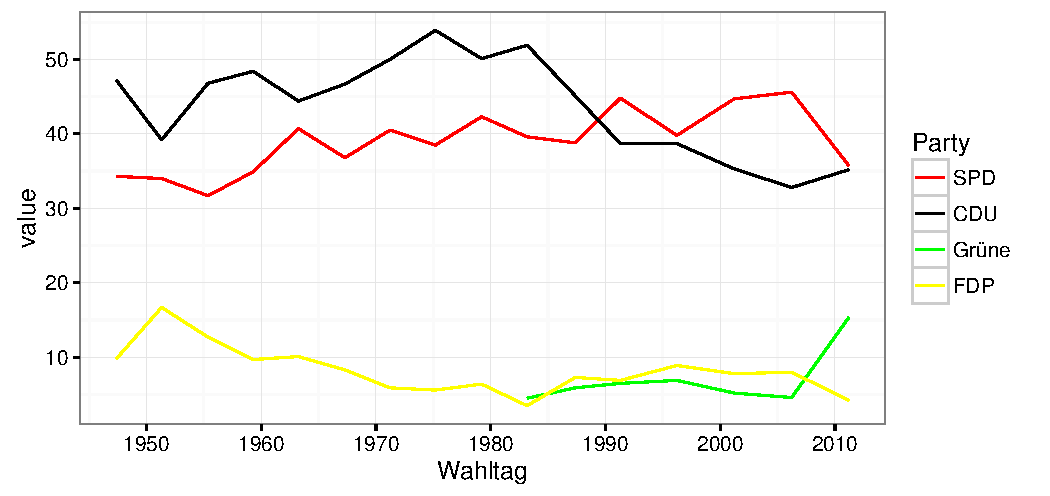
\includegraphics[width=0.7\textwidth]{fig/p1.pdf}
\end{frame}


\section{unstructured webpages}
\subsection{}
\begin{frame}[fragile]
\frametitle{III - Scraping unstructured web-pages}
\begin{itemize}
	\item Not all data is stored in <table>
	\item scattered on the web page
	\item Need to find and extract the parts we need.
\end{itemize}

	\begin{minted}[fontsize=\tiny]{html}
	<h1 id="Top">Formaldehyde</h1>
	<ul>
	<li>
	<strong>
	<a class="external" href="http://goldbook.iupac.org/R05271.html" title="IUPAC definition of relative molecular mass (molecular weight)">Molecular weight</a>
	:
	</strong>
	30.0260
	</li>
	<li>
	<strong>IUPAC Standard InChIKey:</strong>
	<span style="font-family: monospace;">WSFSSNUMVMOOMR-UHFFFAOYSA-N</span>
	</li>
	<li>
	<strong>CAS Registry Number:</strong>
	50-00-0
	</li>
	\end{minted}
\end{frame}


\begin{frame}[fragile]
\frametitle{III - XPath}
XML Path Language (XPath) is a query language for selecting nodes

\end{frame}




\section{Lessons learned}
\subsection{}
\begin{frame}
\frametitle{IV - Remarks}
\begin{itemize}
	\item scraping is easy.
	\item being user-friendly is \textcolor{hilight}{not}.
	\item be nice to the servers!
	\begin{itemize}
		\item scrape slowly, time-outs
		\item Sys.sleep(rgamma(1, shape = 30, scale = 1/10))
	\end{itemize}
	\item illegal?
	\begin{itemize}
		\item even slower
		\item anonymous EC2
		\item TOR
	\end{itemize}
\end{itemize}

\end{frame}



%%% Last slide ----------------------------------------------------
\begin{frame}
    \frametitle{}

    \vspace{1em}
    \begin{centering}
    \Large \textcolor{title}{Web Scraping with R} \\[1em]
        Eduard Szöcs \\[0.3em]
    \tiny \textcolor{gray}{Institute for Environmental Sciences, University of Koblenz-Landau} \\[5em]
    \end{centering}
    \normalsize
    \textcolor{hilight}{\faLaptop}~~~\href{http://edild.github.io/}{http://edild.github.io/ }\\[.5em]
    \textcolor{hilight}{\faGift}~~~\href{https://github.com/edild/talk_webscrapingr}{https://github.com/edild/talk\_webscrapingr}\\[0.5em]
    \textcolor{hilight}{\faTwitter}~~~\href{http://twitter.com/EduardSzoecs}{@EduardSzoecs}     \\[0.5em]
    \textcolor{hilight}{\faEnvelope}~~~\href{mailto:szoecs@uni-landau.de}{szoecs@uni-landau.de} \\[.5em]
    \hfill 
\includegraphics[width =.3\textwidth]{fig/Cc-by-nc_euro_icon.png} 
\end{frame}


\end{document}